\begin{figure}[h]
    \centering
    \begin{subfigure}[b]{0.485\textwidth}
        \centering
        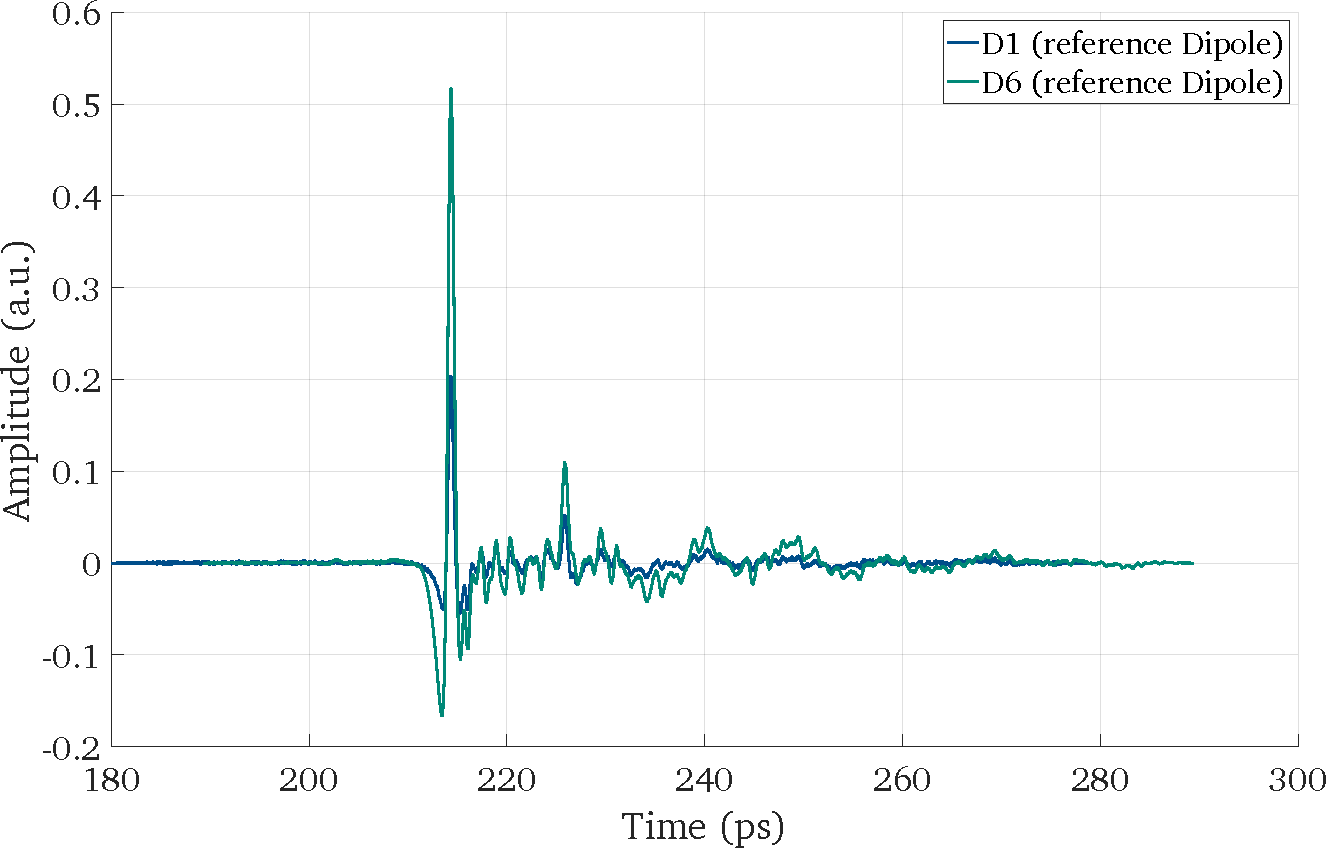
\includegraphics[width=\textwidth]{figures/Results/D1_D6/D1_D6_time.pdf}
        \caption{}
    \end{subfigure}
    \hfill
    \begin{subfigure}[b]{0.485\textwidth}
        \centering
        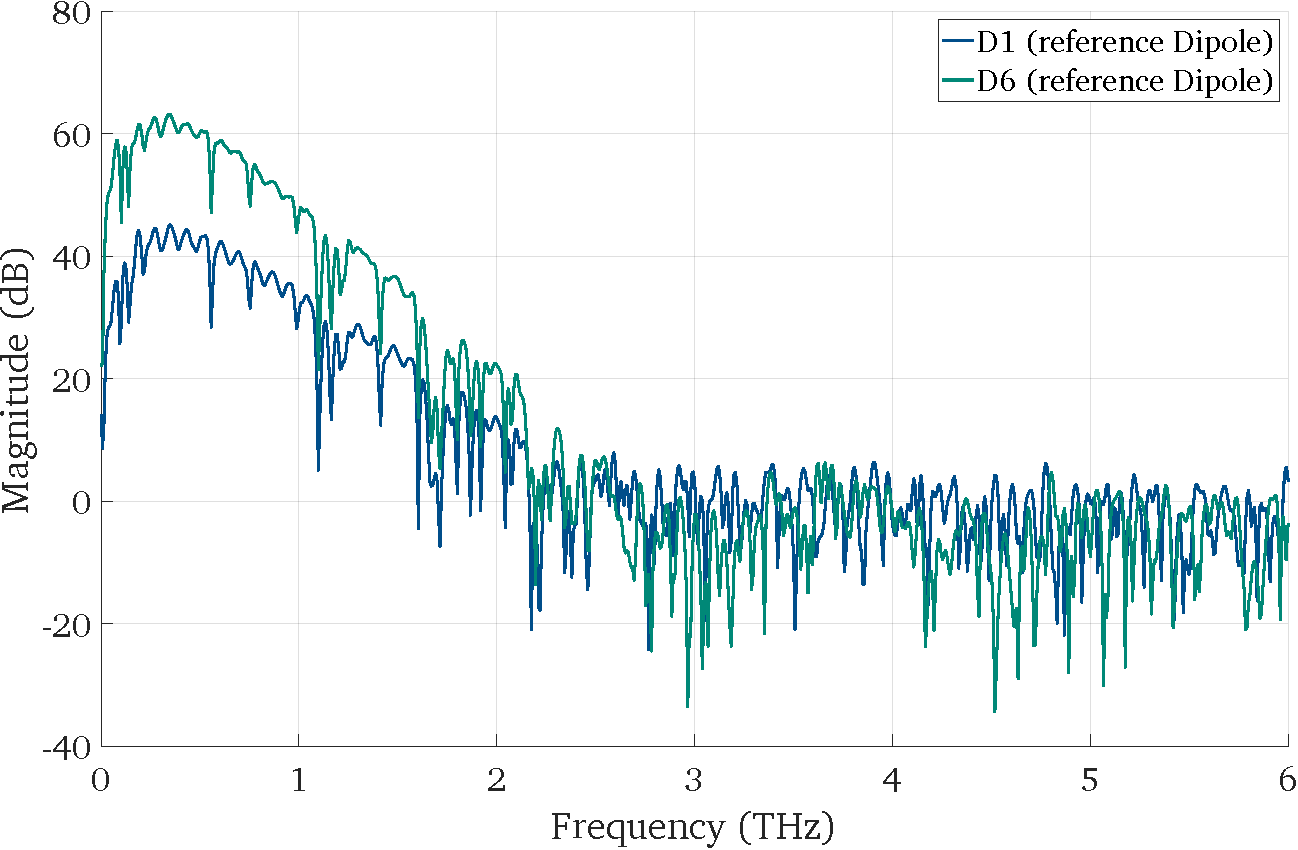
\includegraphics[width=\textwidth]{figures/Results/D1_D6/D1_D6_spectrum_nn.pdf}
        \caption{}
    \end{subfigure}
    \caption{Comparison of two Dipoles with equal topology. (a) Time-domain signal. (b) Spectrum normed to the signals noise floor.}
\end{figure}

\begin{figure}[h]
    \centering
    \begin{subfigure}[b]{0.485\textwidth}
        \centering
        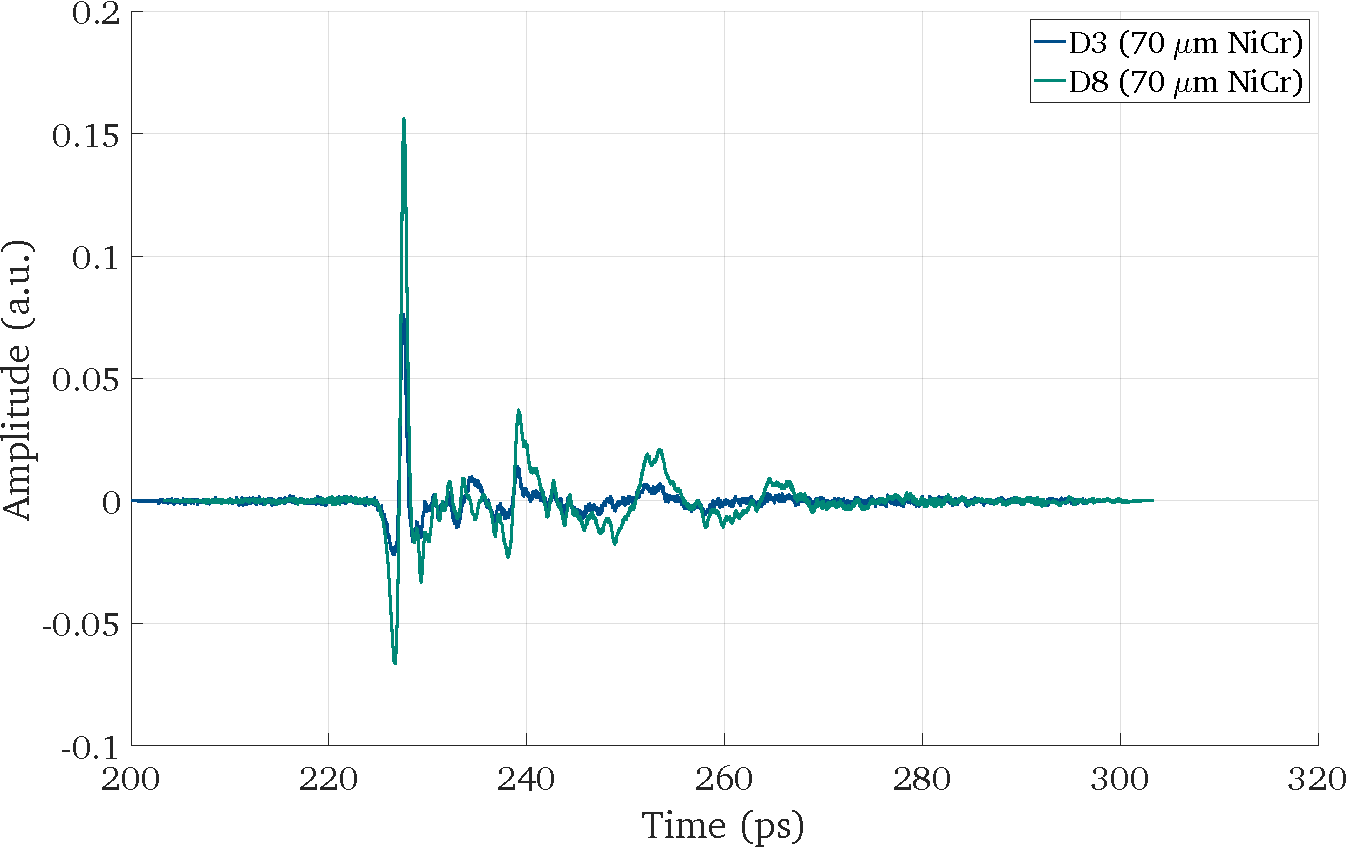
\includegraphics[width=\textwidth]{figures/Results/D3_D8/D3_D8_time.pdf}
        \caption{}
    \end{subfigure}
    \hfill
    \begin{subfigure}[b]{0.485\textwidth}
        \centering
        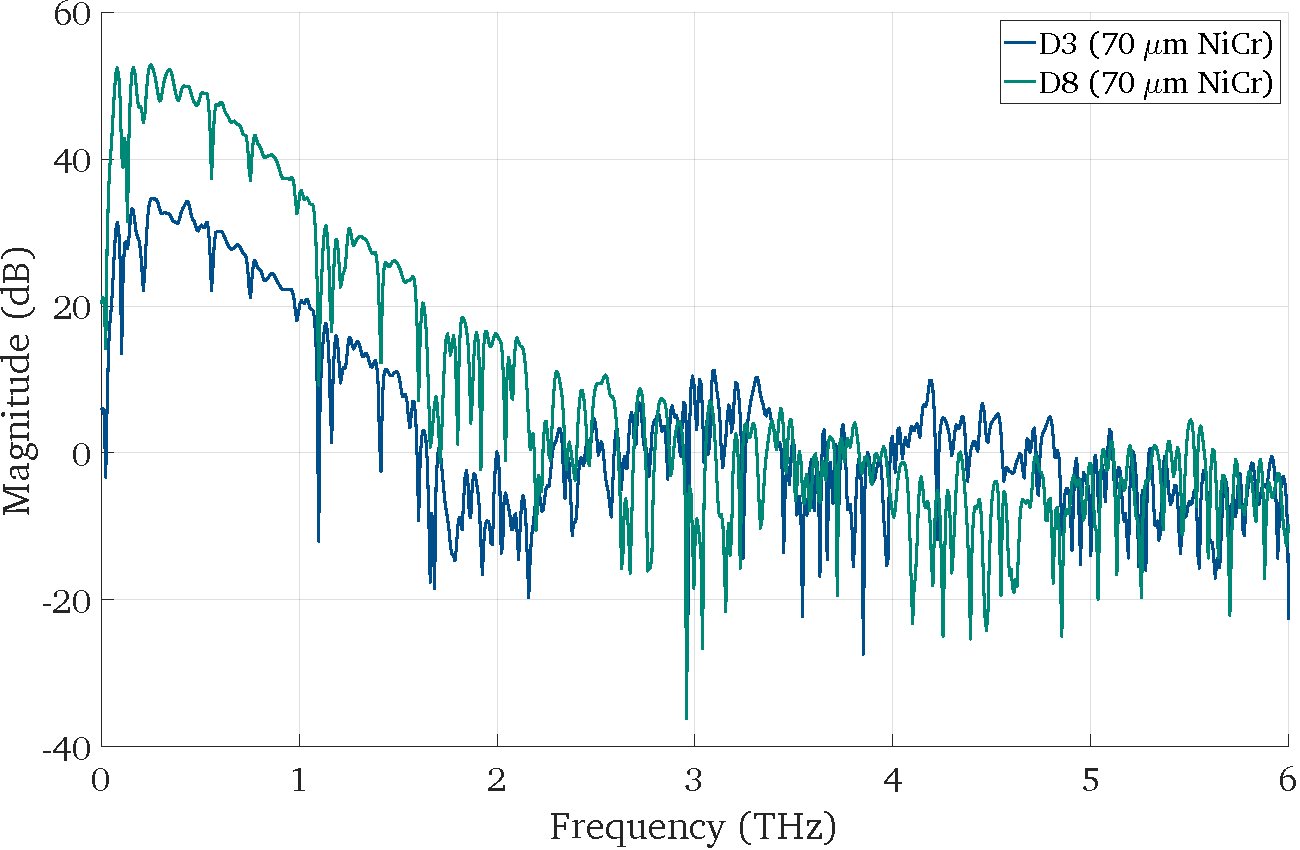
\includegraphics[width=\textwidth]{figures/Results/D3_D8/D3_D8_spectrum_nn.pdf}
        \caption{}
    \end{subfigure}
    \caption{Comparison of two Dipoles with equal topology. (a) Time-domain signal. (b) Spectrum normed to the signals noise floor.}
\end{figure}

\begin{figure}[h]
    \centering
    \begin{subfigure}[b]{0.485\textwidth}
        \centering
        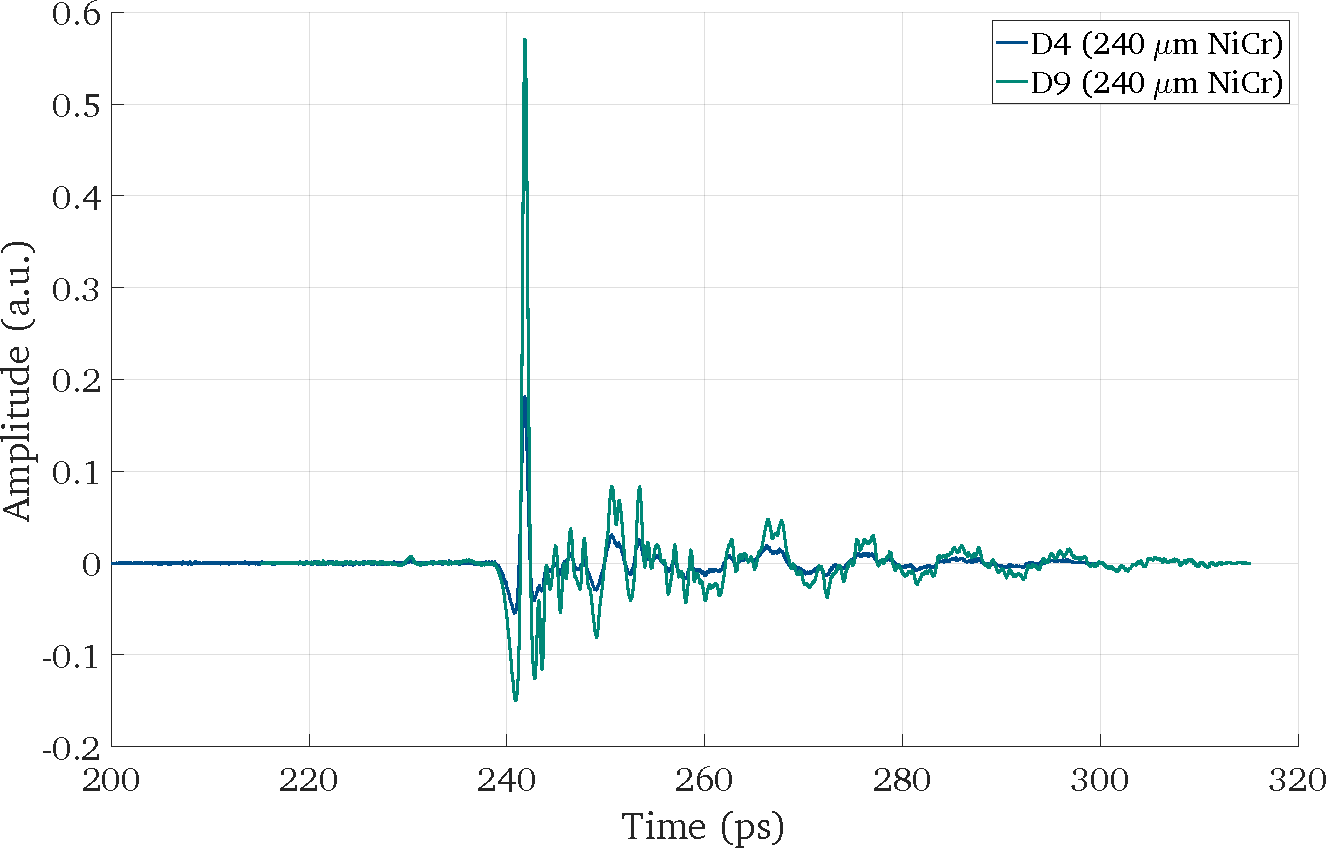
\includegraphics[width=\textwidth]{figures/Results/D4_D9/D4_D9_time.pdf}
        \caption{}
    \end{subfigure}
    \hfill
    \begin{subfigure}[b]{0.485\textwidth}
        \centering
        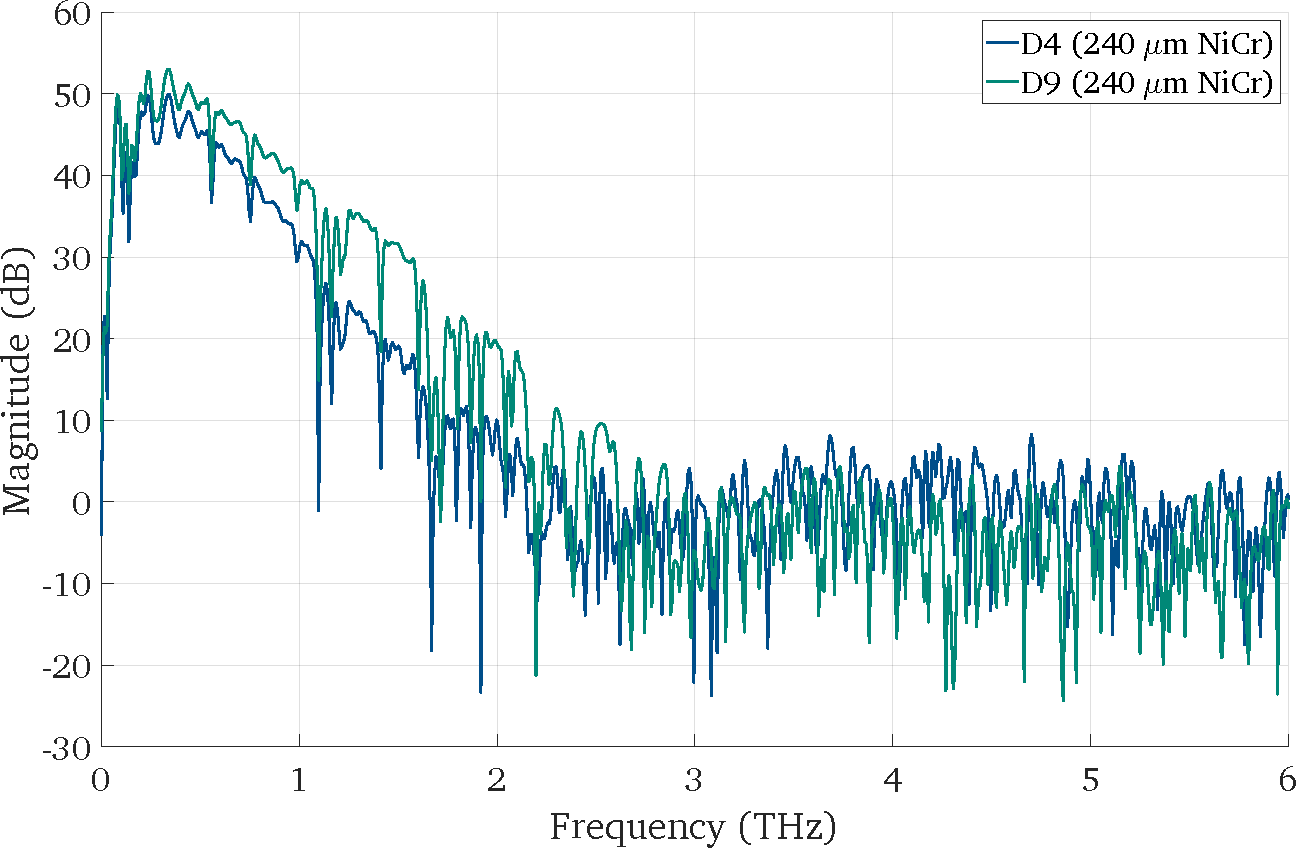
\includegraphics[width=\textwidth]{figures/Results/D4_D9/D4_D9_spectrum_nn.pdf}
        \caption{}
    \end{subfigure}
    \caption{Comparison of two Dipoles with equal topology. (a) Time-domain signal. (b) Spectrum normed to the signals noise floor.}
\end{figure}

\begin{figure}[h]
    \centering
    \begin{subfigure}[b]{0.485\textwidth}
        \centering
        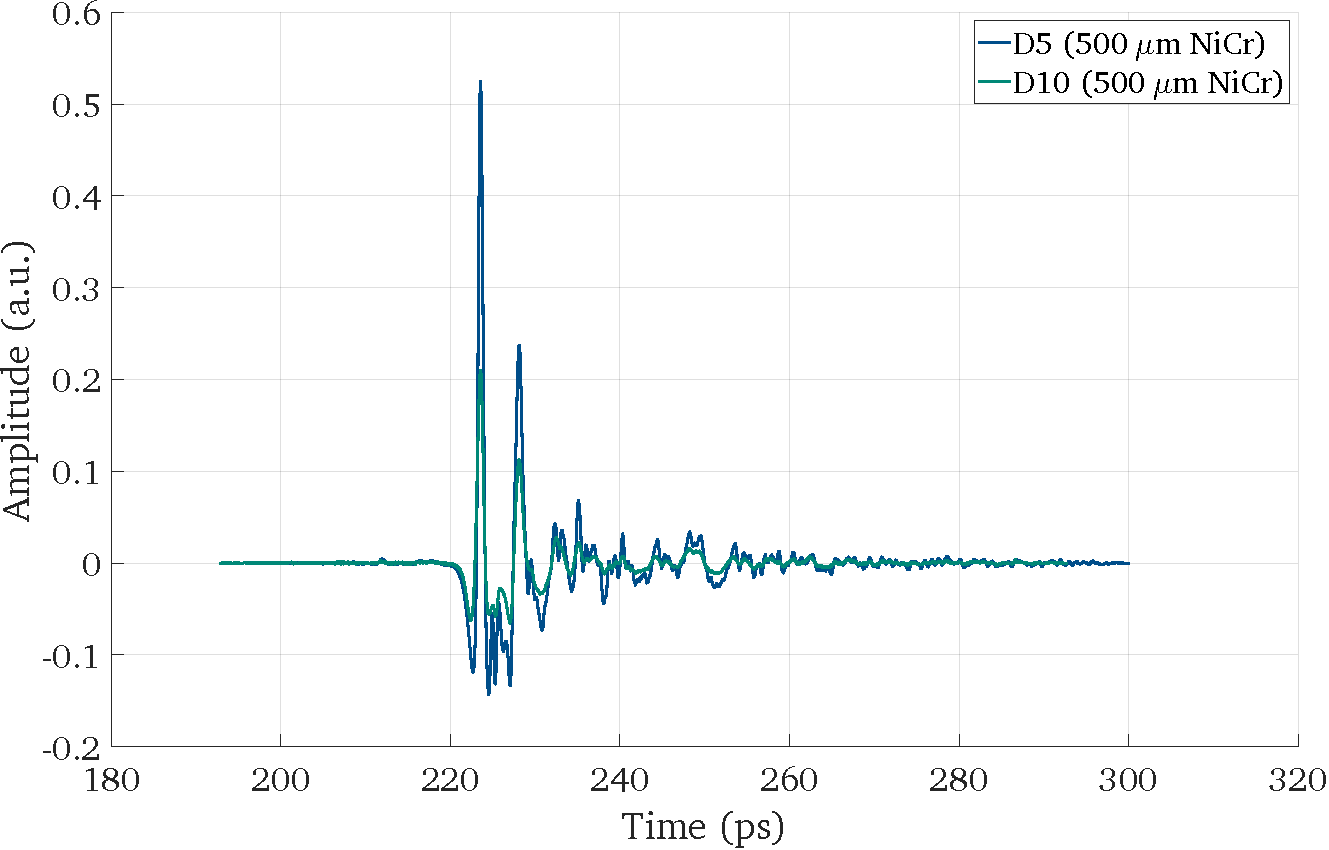
\includegraphics[width=\textwidth]{figures/Results/D5_D10/D5_D10_time.pdf}
        \caption{}
    \end{subfigure}
    \hfill
    \begin{subfigure}[b]{0.485\textwidth}
        \centering
        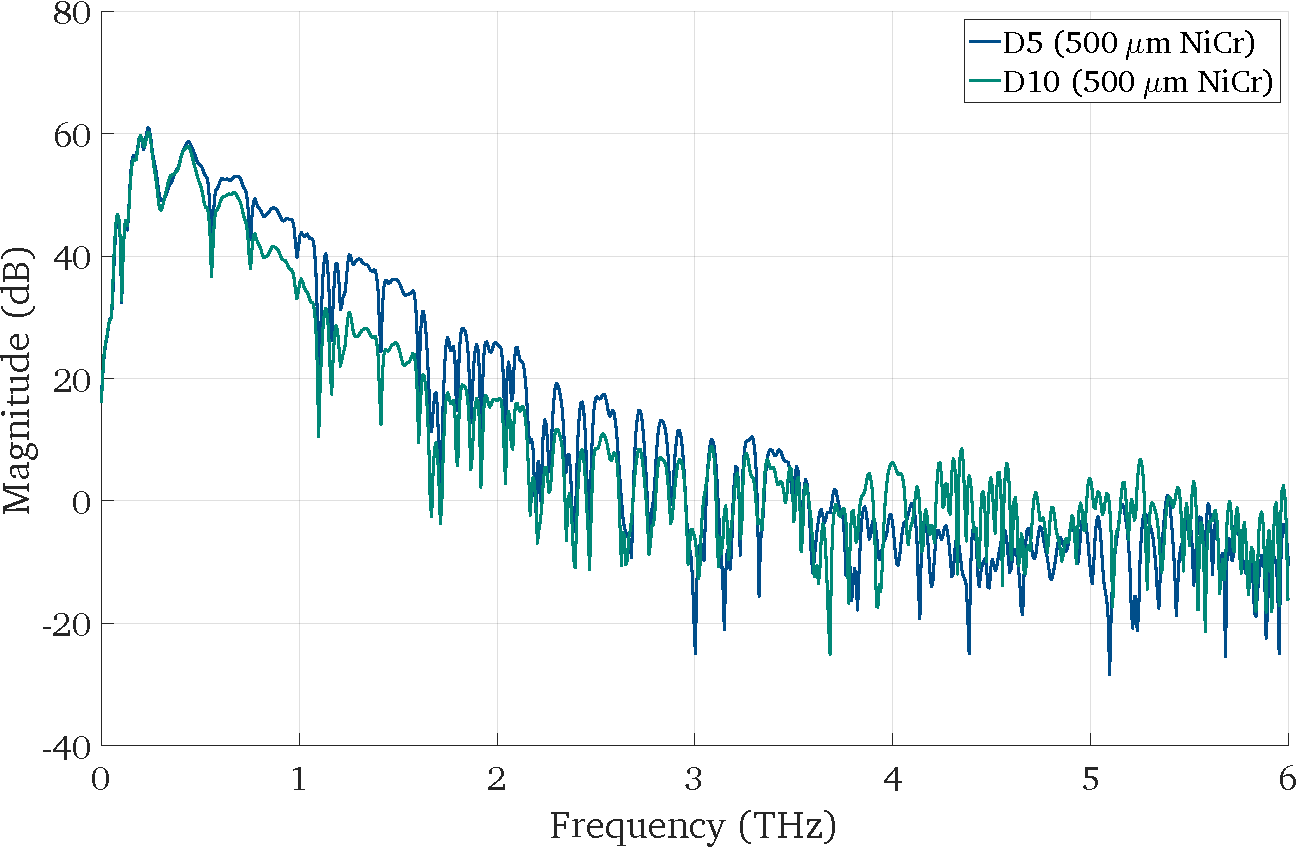
\includegraphics[width=\textwidth]{figures/Results/D5_D10/D5_D10_spectrum_nn.pdf}
        \caption{}
    \end{subfigure}
    \caption{Comparison of two Dipoles with equal topology. (a) Time-domain signal. (b) Spectrum normed to the signals noise floor.}
\end{figure}

\begin{figure}[h]
    \centering
    \begin{subfigure}[b]{0.485\textwidth}
        \centering
        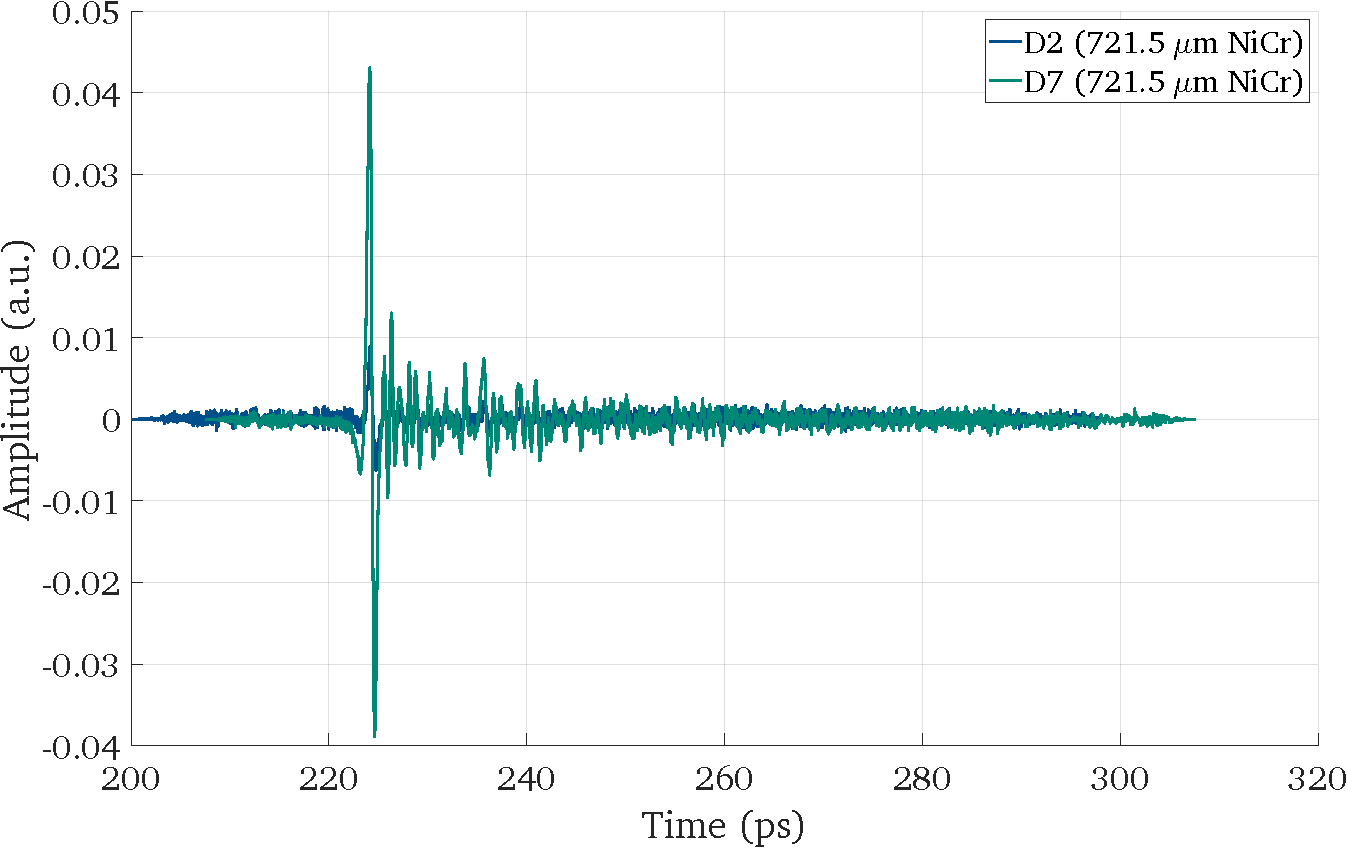
\includegraphics[width=\textwidth]{figures/Results/D2_D7/D2_D7_time.pdf}
        \caption{}
    \end{subfigure}
    \hfill
    \begin{subfigure}[b]{0.485\textwidth}
        \centering
        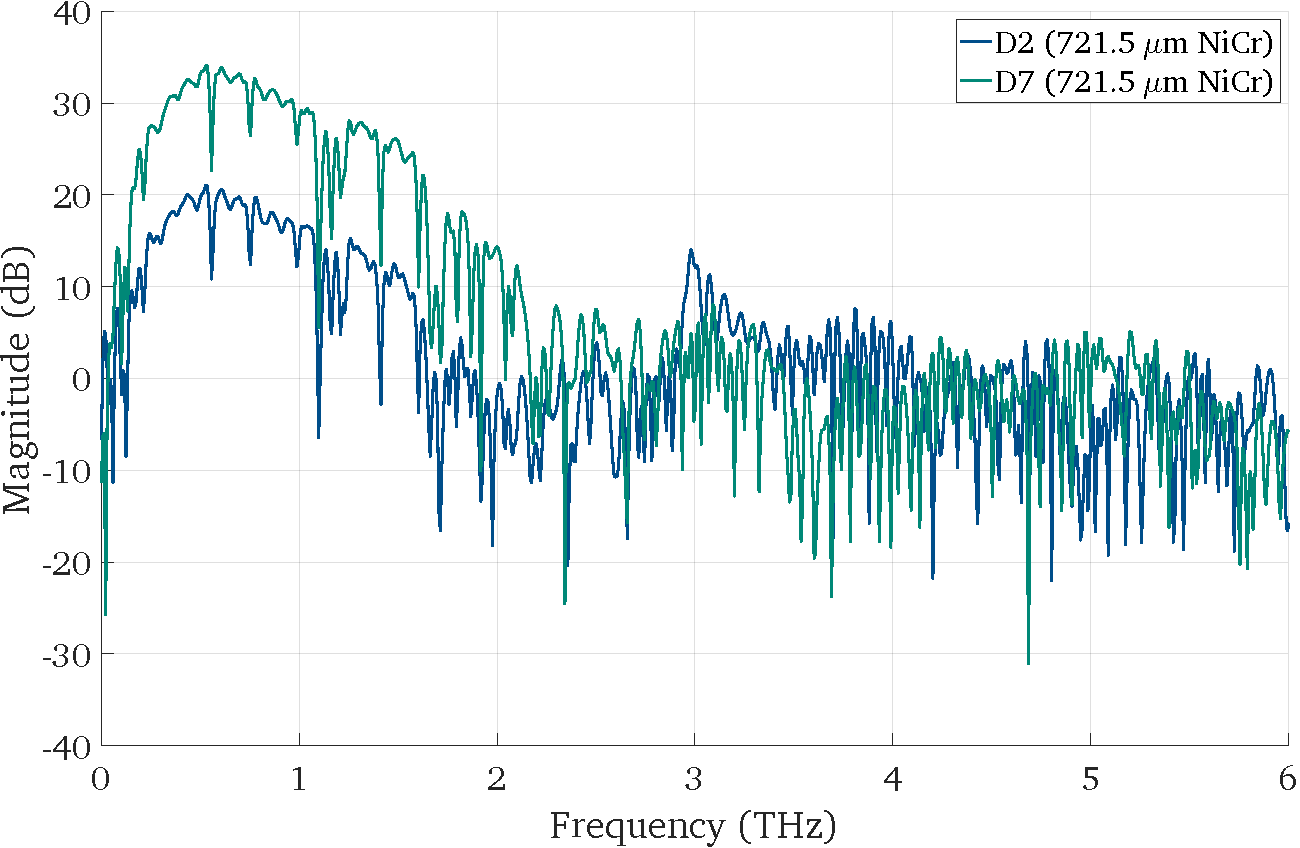
\includegraphics[width=\textwidth]{figures/Results/D2_D7/D2_D7_spectrum_nn.pdf}
        \caption{}
    \end{subfigure}
    \caption{Comparison of two Dipoles with equal topology. (a) Time-domain signal. (b) Spectrum normed to the signals noise floor.}
\end{figure}